\chapter{Arbejdsproces}

I dette projekt har vi anvendt et online v�rkt�j: Scrumwise\footnote{www.scrumwise.com}, til at holde styr p� vores arbejdsproces. Vi har mulighed for at holde styr p� alle arbejdsopgaver l�bende vha. v�rkt�jer i Scrumwise.

Vi har lavet en backlog til vores projekt, som indeholder alle de overordnede opgaver der skal laves over hele projektforl�bet. Disse opgaver er derefter delt ud p� nogle forskellige sprints, hvor de brugere der er tilmeldt det givne projekt har mulighed for at "tage en opgave", s� man undg�r at flere personer arbejder p� det samme modul. Det har v�ret en k�mpe fordel at anvende v�rkt�jer som dette, da det giver os et overblik over hele projektet, sprints og konkrete kode-moduler.

I de fire f�rste sprints har vi afsluttet tre backlog-opgaver, som det ses nedenfor p� figuren. Det er herefter muligt at tilf�je en eller flere backlog-opgaver til fremtidige sprints, hvor det er planen at afslutte de tre sidste opgaver over den sidste tid der er til r�dighed inden den endelige applikation skal st� f�rdig.

\begin{figure}[H]
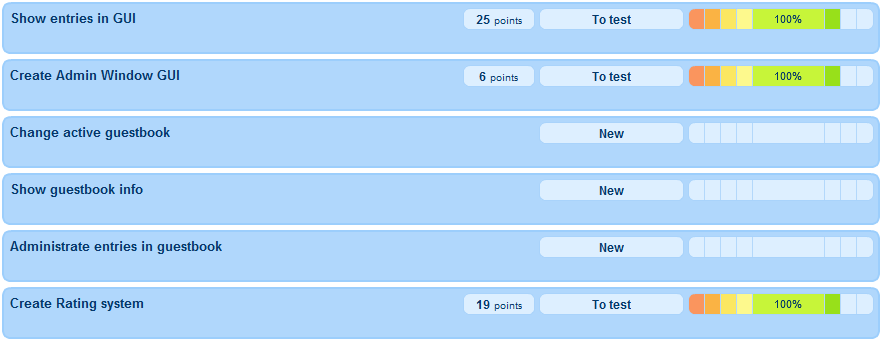
\includegraphics[width=\linewidth]
{./Backlog}
\caption{Backlog for projektet}
\label{Backlog}
\end{figure}

Sprint fire gik ud p� at optimere funktionaliteten af vores forhenv�rende applikation. Heriblandt er det nu muligt at tilf�je en vurdering i form at stjerner, p� en skala fra 1-5, som bliver tilknyttet en g�stebogsbesked. Derudover er fanebladet hvor man kan se g�stebogsbeskeder blevet optimeret i form af en mere dynamisk l�sning. Der bliver nu tilf�jet/fjernet sider i g�stebogen alt efter hvor mange beskeder der er tilknyttet hver side. Hvis der er mere end fem beskeder vil der automatisk blive oprettet en ny side, og en knap der g�r det muligt at g� videre til n�ste side blive aktiveret, samt en tilbage-knap hvis man er p� en anden side end den f�rste. Til sidst er der blevet �ndret nogle sm�-ting i koden og UI'et, s� det hele er optimeret.

Arbejdsmoralen har i dette sprint v�ret ekspotientielt, grundet lidt svingende frav�r og helbred. Som det fremg�r af burndown-figuren tog det os lang tid at planl�gge hvilke arbejdsopgaver der skulle konstrueres i dette sprint. Dog var det muligt for os at n� at lave alle opgaver f�rdig til deadline fredag, da vi tog en t�rn midt p� ugen.

\begin{figure}[H]
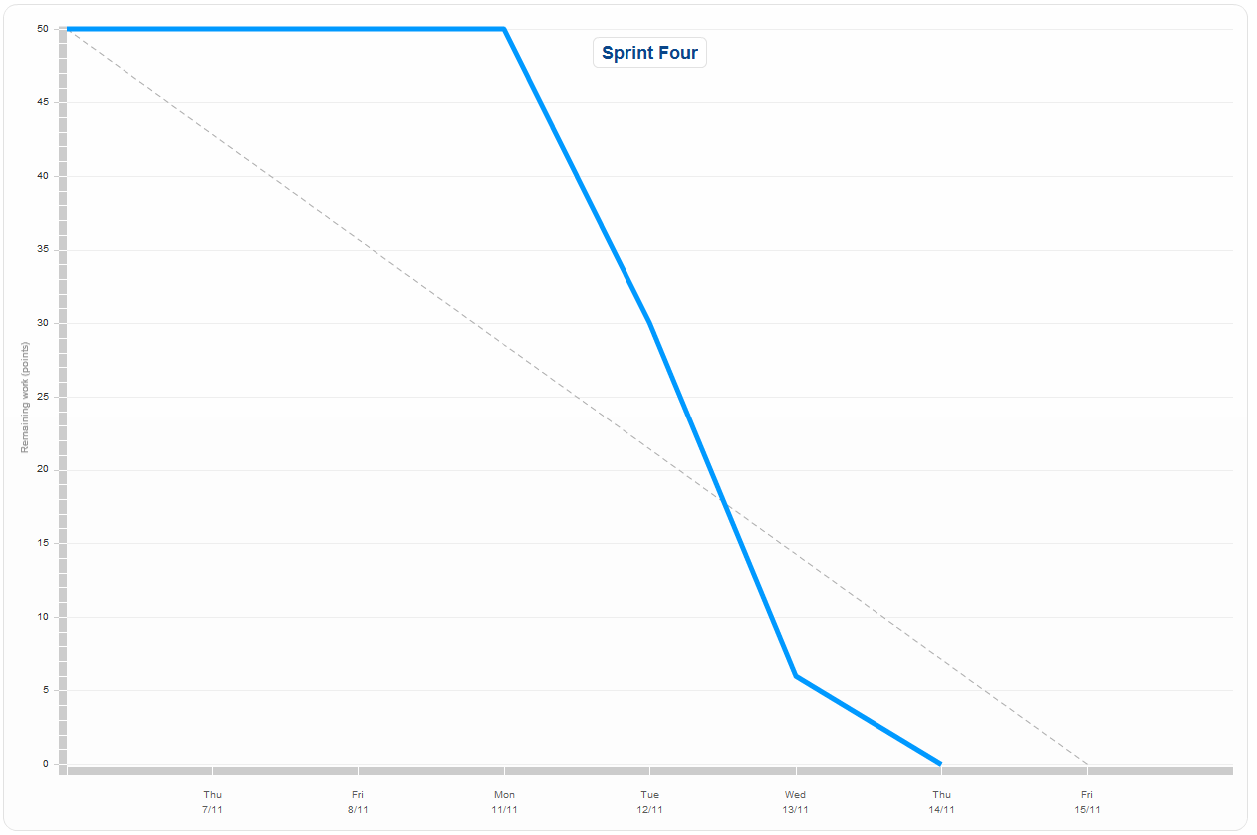
\includegraphics[width=\linewidth]
{./Burndown}
\caption{Burndown for sprint fire}
\label{Burndown chart}
\end{figure}